%% Q1
The best definition of education is that it \textbf{prepares autonomous human beings}: individuals who think, judge and act independently and responsibly. Social change, useful knowledge and employment are only by-products.

%% Q2
The semester system provides \textbf{scope for continual appraisal}: frequent assessment, feedback and course correction within shorter learning units, per the official key.

%% Q3
Making students own responsibility for learning means the teacher \textbf{helps students evolve their own ways of learning}, so that they become self-directed, independent learners.

%% Q4
Emphasis on ``how'' and ``how well'' students learn reflects the idea of \textbf{learning to learn}, i.e.\ developing metacognition and lifelong learning skills. (Compare the Delors Report's four pillars: learning to know, to do, to live together, to be.)

%% Q5
Assessment only at the end of term is less useful because it may capture \textbf{temporary learning} (crammed and soon forgotten) rather than lasting understanding. Continuous assessment gives a truer picture.

%% Q6
From least to most difficult: teaching \textbf{processes (1)} $\rightarrow$ \textbf{concepts (3)} $\rightarrow$ \textbf{thinking skills (4)} $\rightarrow$ \textbf{values (2)}. Values are the hardest because they involve the affective domain and must be internalised.

%% Q7
Gujarat set up a separate board (Admission Committee for Professional Courses / the regulatory board under the Gujarat Professional \textbf{Technical} Educational Colleges or Institutions Act, 2007) to regulate admissions and fees of \textbf{technical} education institutions, per the key.

%% Q8
Progressive institutions cope with rising numbers by using multimedia across \textbf{ODL, face-to-face, satellite and web-based modes}, i.e.\ blended and multi-mode delivery.

%% Q9
Graduates are expected to be \textbf{sensitive and proactive towards emerging concerns and issues} of society and the nation, not merely job-seekers.

%% Q10
The \textbf{UGC} frames regulations and guidelines for maintaining standards in universities and colleges (UGC Act, 1956, Section 12). NAAC only assesses and accredits.

%% Q11
The national open university is \textbf{Indira Gandhi National Open University (IGNOU)}, New Delhi (1985).

%% Q12
Per the key, the three kinds are \textbf{State Universities, Central Universities and Deemed-to-be Universities} (with private universities being added later).

%% Q13
A characteristic that can take different values or categories is a \textbf{variable}; one that cannot vary is a constant.

%% Q14
Studying the relationship between gender and intelligence in a population of students, as they exist without manipulation, is a \textbf{survey (descriptive--correlational) study}.

%% Q15
Per the key, a \textbf{pie chart} best shows how a whole is divided among the different levels (categories) of a variable.

%% Q16
\textbf{Reliability} is the \textbf{consistency} (stability) of test scores. Appropriateness of interpretations is \emph{validity}.

%% Q17
Teachers who personally taught the new maths are eye-witnesses, so they are \textbf{primary sources}.

%% Q18
In a \textbf{positive correlation} both variables move in the \textbf{same direction} (both increase or both decrease).

%% Q19 ctx
\textbf{Directions (Q.~Nos.~19 to 21):} Given data tabulates admission (in percentage) of the candidates to the four courses in five years from 1991 to 1995.
\begin{center}\small
\begin{tabular}{lcccc}\toprule \textbf{Year} & \textbf{Biology} & \textbf{Geology} & \textbf{Chemistry} & \textbf{Mathematics}\\\midrule
1991 & 35 & 30 & 20 & 15\\ 1992 & 40 & 35 & 15 & 10\\ 1993 & 30 & 25 & 20 & 25\\ 1994 & 20 & 20 & 30 & 30\\ 1995 & 30 & 30 & 25 & 15\\\bottomrule
\end{tabular}
\end{center}

%% Q19
Chemistry: 1993 $=20\%$, 1994 $=30\%$. Increase $=\dfrac{30-20}{20}\times100=\mathbf{50\%}$.

%% Q20
Biology: 1992 $=40\%$, 1993 $=30\%$. Fall $=\dfrac{40-30}{40}\times100=\mathbf{25\%}$.

%% Q21
1993: Biology 30, Geology 25, \textbf{Chemistry 20}, Mathematics 25. The least is Chemistry.

%% Q22 ctx
\textbf{Directions (Q.~Nos.~22 to 24):} The following data provides the information of outgoing students from an academic institution after completing their study.
\begin{center}\small
\begin{tabular}{lccc}\toprule \textbf{Percentage of students} & \textbf{2003} & \textbf{2004} & \textbf{2005}\\\midrule
by campus recruitment & 33 & 38 & 39\\ in further study & 40 & 36 & 37\\ unemployed & 2 & 1 & 3\\ to other activities & 25 & 25 & 22\\\midrule
Total number of students & 1200 & 1100 & 1000\\\bottomrule
\end{tabular}
\end{center}

%% Q22
Campus recruitment: 2003 $=33\%\times1200=396$; 2004 $=38\%\times1100=\mathbf{418}$; 2005 $=39\%\times1000=390$. The largest is 418.

%% Q23
Further studies: 2003 $=40\%\times1200=480$; 2005 $=37\%\times1000=370$. Decrease $=\mathbf{110}$.

%% Q24
Other activities in 2004 $=25\%\times1100=\mathbf{275}$.

%% Q25 ctx
\textbf{Directions (Q.~Nos.~25 to 30):} Read the following text and answer the questions.\par\smallskip
The world is becoming global rapidly. The national boundaries have become less significant with the interlinked effects of technology, information flows and investment mobility. Human knowledge, particularly in the sphere of science and technology, is now growing at a pace which was indeed unthinkable even two decades ago. The comparative advantage of a nation will be more and more influenced by its capacity to generate, absorb, adapt and assimilate new technologies into production process. If liberalisation and globalisation are not to create islands of prosperity surrounded by vast sea of destitution, there has to be firm commitment to human resource development and to continuous upgrading of human skills and capabilities in the fast changing world that we live in. The Indian policy makers are fully committed to building a society which is technologically sophisticated, economically progressive and socially just and humane.

Impact of globalisation on education is now being felt in India. Indian entrepreneurs are also now investing in education. In the process of privatisation of higher education in India, many good institutions have come up and have met the increasing demand for higher education mainly in the area of engineering, business administration and medical education. But this process has also led to mushroom growth of low quality institutions without proper infrastructure. However, the expansion of higher education in India has resulted in increasing access to higher education even in rural areas of the country. In this process, Human Resource Development is taking place at a faster speed as compared to the earlier stage when the opportunities for higher education were limited.

Globalisation has promoted information technology in India. Indian students have excelled in the area of information technology over many other countries. Developments taking place in the developed countries become available to Indian students, scholars and practitioners through regular contacts and through the modern technology.

%% Q25
New technology makes developments in the developed countries available to Indian students, so they can \textbf{study IT in India} itself (``through regular contacts and through the modern technology'').

%% Q26
``In the process of \textbf{privatisation of higher education} \ldots\ Human Resource Development is taking place at a faster speed.''

%% Q27
Firm commitment is needed so that globalisation does not create ``islands of prosperity surrounded by vast sea of destitution'', i.e.\ to spread prosperity, reduce destitution and upgrade human skills. \textbf{All of the above}.

%% Q28
The passage names technology, information flows, investment mobility and rapid growth of knowledge. ``\textbf{Generation of new technologies}'' is given by the key as \emph{not} a factor of speed; the passage mentions the capacity to generate technology as a source of a nation's comparative advantage, not as a driver of globalisation's speed.

%% Q29
Without a just and humane society, liberalisation and globalisation would ``create islands of prosperity surrounded by vast sea of destitution'', i.e.\ \textbf{economic imbalance}.

%% Q30 q
Find out the results of privatization of education in India, from the following:\\
(1) Higher education has become accessible to rural students.\\
(2) The pace of human resource development has increased.\\
(3) Many low quality colleges have come up.\\
(4) The quality of medical and engineering education has improved a lot.

%% Q30
The passage states (1) access in rural areas has increased, (2) HRD is faster, and (3) low-quality institutions have mushroomed. It does not claim (4). The answer is \textbf{(1), (2) and (3)}.

%% Q31
\textbf{EDUSAT} (GSAT-3, launched by ISRO in 2004) was India's first satellite dedicated exclusively to \textbf{educational} transmission.

%% Q32
Teachers should not only communicate effectively but also \textbf{develop effective communication in students}.

%% Q33
\textbf{Many-to-many} communication (all members interacting, as in discussion) is the most preferable in class, being interactive and participatory.

%% Q34
Nodding while listening signals attention and approval, i.e.\ it \textbf{encourages} the speaker to continue.

%% Q35
Per the key, \textbf{copying down points from the blackboard} is a mechanical activity rather than a communicative situation (no exchange of meaning takes place).

%% Q36
The major barrier is \textbf{lack of perceptible feedback} from the receiver: without it the sender cannot know whether the message was understood.

%% Q37
A website's address is its \textbf{URL} (Uniform Resource Locator).

%% Q38
To end an Internet session one must \textbf{log out}.

%% Q39
A \textbf{.pdf} file is designed for viewing and printing with fixed layout. It is not normally editable without special software, unlike .doc, .ppt and .txt.

%% Q40
A virus is software and can delete files, corrupt programs and even crash disks (by corrupting data). It cannot physically damage the \textbf{motherboard} hardware.

%% Q41
``Internet'' comes from \textbf{inter-connection} (interconnected) \textbf{network}: a network of networks.

%% Q42
\textbf{HTML} is \textbf{HyperText Markup Language}.

%% Q43
The value equals the position of the \textbf{last letter}: HOW $\rightarrow$ W $=23$, HAI $\rightarrow$ I $=9$, so SEX $\rightarrow$ X $=\mathbf{24}$.

%% Q44
The differences are odd numbers: $+1, +3, +5, +7, +9$, giving $3, 4, 7, 12, \mathbf{19}, 28$.

%% Q45
A set with $n$ elements has $2^n$ subsets. Here $n=6$, so $2^6=\mathbf{64}$.

%% Q46 q
Choose the correct answer to complete the sequence:

%% Q46 fig
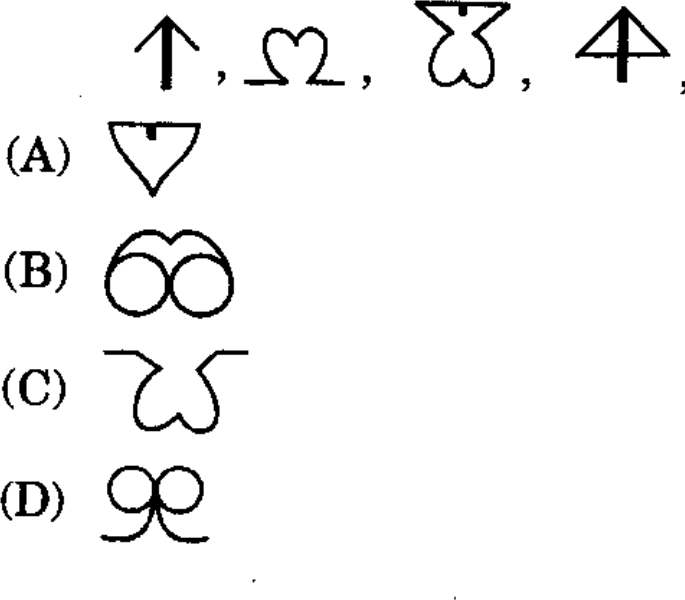
\includegraphics[height=3.6cm]{fig/oct10_q46.png}

%% Q46 opts
Figure (A)
Figure (B)
Figure (C)
Figure (D)

%% Q46
Each figure is a \textbf{digit joined with its own mirror image}: 1 and its mirror give $\uparrow$, 2 and its mirror give the second shape, then 3 and 4. The next figure must be \textbf{5 joined with its mirror image}, which is figure (C).

%% Q47
Replace the symbols: $[\{(4\times3)\div2\}^2]\div(6^0)=[6^2]\div1=36$.
36 is not among the options, so the agency \textbf{dropped} the question.

%% Q48
The rule is $x\mapsto x^3-4$: $0-4=-4$, $1-4=-3$, $8-4=4$, $27-4=23$.
\[\left(\tfrac34\right)^3-4=\frac{27}{64}-4=\frac{27-256}{64}=-\frac{229}{64}\]

%% Q49
Z $>$ V $>$ X $>$ W $>$ Y, so \textbf{Z} is the tallest.

%% Q50
Positions decrease by 4: x(24), \textbf{t(20)}, p(16), l(12), h(8).

%% Q51 opts
\tikz[baseline=-0.5ex,scale=0.3]{\draw (0,0) circle(1.3); \draw (-0.6,0) circle(0.35); \draw (0.6,0) circle(0.4); \draw (0.6,0) circle(0.2);}
\tikz[baseline=-0.5ex,scale=0.3]{\draw (0,0) circle(1.3); \draw (0,0.7) circle(0.3); \draw (-0.6,-0.3) circle(0.3); \draw (0.6,-0.3) circle(0.3);}
\tikz[baseline=-0.5ex,scale=0.3]{\draw (0,0) circle(1.3); \draw (0,0) circle(0.85); \draw (-0.3,0) circle(0.25); \draw (0.3,0) circle(0.25);}
None of (A), (B), (C)

%% Q51
The \textbf{school} contains the \textbf{classroom}, and inside the classroom are the \textbf{teacher} and the \textbf{blackboard} (two separate things). So two small separate circles lie inside the classroom circle, which lies inside the school circle, as in diagram (C).

%% Q52 q
Fill the correct letter from the given alternatives, in place of question-mark:\\[3pt]
\centering\begin{tabular}{ccc}
\begin{tabular}{|c|c|}\hline C & H\\\hline\multicolumn{2}{|c|}{E}\\\hline R & M\\\hline\end{tabular} &
\begin{tabular}{|c|c|}\hline A & G\\\hline\multicolumn{2}{|c|}{F}\\\hline S & M\\\hline\end{tabular} &
\begin{tabular}{|c|c|}\hline H & J\\\hline\multicolumn{2}{|c|}{?}\\\hline N & L\\\hline\end{tabular}\\
\end{tabular}

%% Q52
The centre letter's position is the difference between the two top letters:
H(8) $-$ C(3) $=5=$ E; G(7) $-$ A(1) $=6=$ F; J(10) $-$ H(8) $=2=$ \textbf{B}.

%% Q53 q
Put the correct letter in the diagram, from the given alternatives, to replace `?':\\[3pt]
\centering
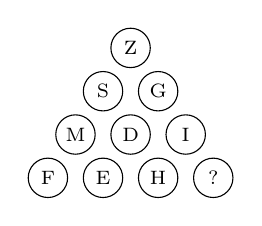
\begin{tikzpicture}[every node/.style={circle,draw,inner sep=1pt,minimum size=5mm,font=\scriptsize}]
\node at (0,0) {Z}; \node at (-0.35,-0.55) {S}; \node at (0.35,-0.55) {G};
\node at (-0.7,-1.1) {M}; \node at (0,-1.1) {D}; \node at (0.7,-1.1) {I};
\node at (-1.05,-1.65) {F}; \node at (-0.35,-1.65) {E}; \node at (0.35,-1.65) {H}; \node at (1.05,-1.65) {?};
\end{tikzpicture}

%% Q53
The positions in every row add up to 26 (Z):
\[\text{S}(19)+\text{G}(7)=26,\quad \text{M}(13)+\text{D}(4)+\text{I}(9)=26\]
\[\text{F}(6)+\text{E}(5)+\text{H}(8)+?=26\Rightarrow ?=7=\mathbf{G}\]

%% Q54 q
Complete the sequence of squares by choosing the correct figure from the given alternatives:

%% Q54 fig
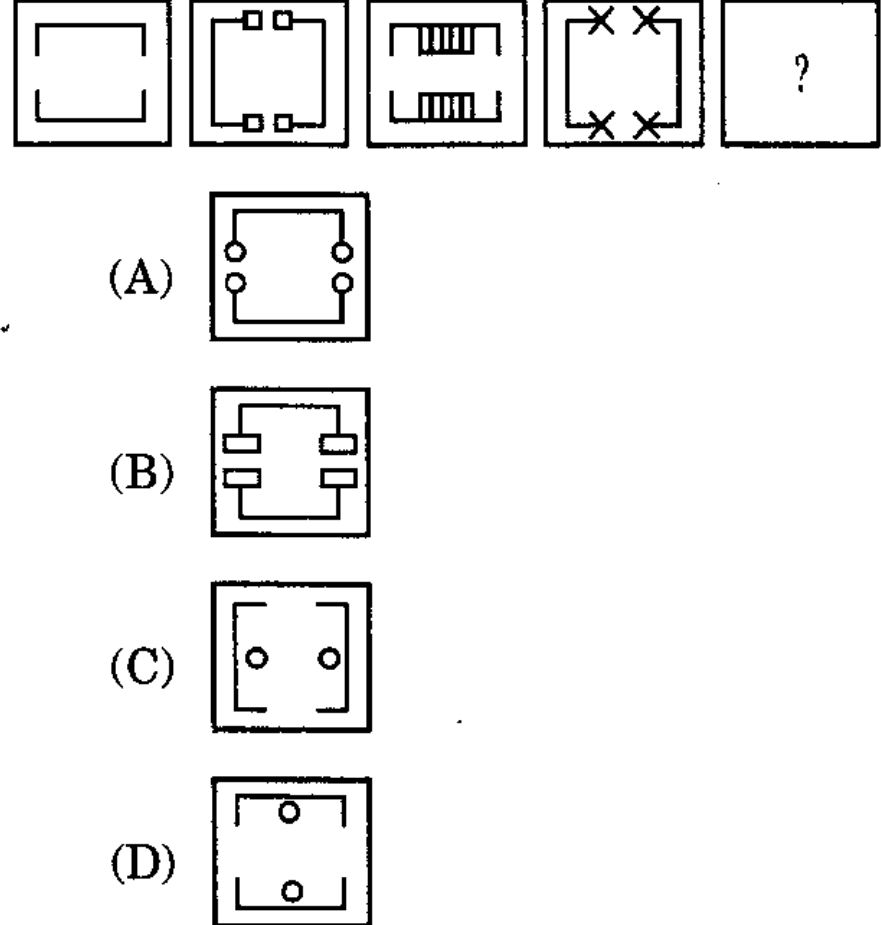
\includegraphics[height=4.6cm]{fig/oct10_q54.png}

%% Q54 opts
Figure (A)
Figure (B)
Figure (C)
Figure (D)

%% Q54
Two changes alternate. The inner frame alternates between being open on the \emph{sides} and open at the \emph{top and bottom}, and a new decoration appears each time on the \textbf{top and bottom} arms (small squares, hatching, crosses). The fifth figure must again have the frame open like the first and third, with a new element (small circles) on the top and bottom arms, which is figure (D).

%% Q55
\textbf{Carbon monoxide} is the most acutely toxic of these gases. It binds to haemoglobin about 200 times more strongly than oxygen, forming carboxyhaemoglobin and causing suffocation.

%% Q56
Per the key, the chief hazard is \textbf{a disaster in a nuclear plant} (accidents such as Chernobyl 1986 and Fukushima 2011), which releases radioactivity over wide areas.

%% Q57
The greenhouse effect is increasing because the \textbf{concentration} of greenhouse gases (CO$_2$, CH$_4$, N$_2$O) in the atmosphere is rising.

%% Q58
Composition of dry air: \textbf{Nitrogen (78\%) $>$ Oxygen (21\%) $>$ Argon (0.93\%) $>$ CO$_2$ ($\approx$0.04\%)}, i.e.\ (2)--(1)--(4)--(3).

%% Q59
Global warming can be reduced by \textbf{increased plantation} (carbon sinks) \textbf{and reduced use of fossil fuels} (fewer emissions), i.e.\ (A) and (C).

%% Q60
Per the key, after CO$_2$ the important greenhouse gas named is \textbf{chlorofluorocarbons (CFCs)}, which have a global-warming potential thousands of times that of CO$_2$.
\tip{By total contribution to warming, methane is usually ranked second after CO$_2$; CFCs are notable for their very high GWP per molecule.}
